%File: main.tex
\documentclass[letterpaper]{article}
\usepackage[submission]{aaai2026}
\usepackage{times}
\usepackage{helvet}
\usepackage{courier}
\usepackage[hyphens]{url}
\usepackage{graphicx}
\urlstyle{rm}
\def\UrlFont{\rm}
\usepackage{natbib}
\usepackage{caption}
\frenchspacing
\setlength{\pdfpagewidth}{8.5in}
\setlength{\pdfpageheight}{11in}
\usepackage{algorithm}
\usepackage{algorithmic}
\usepackage{amsmath,amssymb}
\usepackage{booktabs}
\usepackage{multirow}
\pdfinfo{/TemplateVersion (2026.1)}
\setcounter{secnumdepth}{2}
\newcommand{\method}{FedSSL-MERC}
\newcommand{\ecr}{ECR}
\newcommand{\eafa}{EAFA}

\title{Federated Semi-Supervised Emotion Recognition in Conversations \\
via Evidential Consistency Regularization}
\author{Anonymous Submission}
\affiliations{Anonymous}

\begin{document}
\maketitle

\begin{abstract}
Emotion Recognition in Conversations (ERC) faces two key deployment challenges:
(1) conversational data cannot be centralized due to privacy constraints, and
(2) utterance-level annotations are expensive, leaving most data unlabeled.
We propose \textbf{\method{}}, a federated semi-supervised learning framework
introducing two contributions. \textbf{Evidential Consistency Regularization (\ecr{})}
replaces FixMatch's fragile pseudo-label threshold with certainty-weighted
KL-divergence between Dirichlet distributions from weak and strong augmented views,
avoiding confirmation bias while leveraging epistemic uncertainty from Evidential
Deep Learning. \textbf{Evidential-Aware Federated Averaging (\eafa{})} weights
client aggregation by inverse uncertainty, reducing noisy client influence.
Across 507 experiments on MELD and IEMOCAP with 5 random seeds, ECR consistently
outperforms FixMatch and SOTA baselines (CoMPM, SPCL) on MELD under all label
regimes, achieving \textbf{62.86\% WF1} at 5\% labels with the lowest variance.
Combined ablation confirms ECR as the primary performance driver (+0.47\%).
\end{abstract}

% ================================================================
\section{Introduction}

Emotion Recognition in Conversations (ERC) classifies the emotion of each utterance
within a dialogue, leveraging contextual cues from conversation flow and speaker
interactions \cite{poria2019emotion}. Recent advances using attention architectures
\cite{majumder2019dialoguernn,ghosal2019dialoguegcn} and pre-trained language models
\cite{lee2022compm,song2022spcl} have achieved impressive centralized results but
face two fundamental deployment barriers.

\textbf{Privacy constraints.} Conversational data in healthcare, customer service,
and counseling contains sensitive information protected by regulations (GDPR, HIPAA),
prohibiting centralization and requiring distributed learning \cite{mcmahan2017communication}.

\textbf{Label scarcity.} Utterance-level emotion annotation requires trained
annotators, achieves only moderate inter-annotator agreement ($\kappa \approx
0.48$--$0.58$ for IEMOCAP \cite{busso2008iemocap}), and is prohibitively expensive
at scale. In practice, only 5--10\% of utterances may carry reliable labels.

Federated Learning (FL) \cite{mcmahan2017communication} and Semi-Supervised Learning
(SSL) \cite{sohn2020fixmatch} address these challenges individually, but their
intersection---\textit{federated semi-supervised ERC}---remains under-explored.
The combination of Non-IID emotion distributions, variable speaker demographics,
and dialogue-level dependencies creates challenges absent in standard image
classification benchmarks \cite{jeong2021federated}.

We identify a critical weakness in applying FixMatch \cite{sohn2020fixmatch} to
federated ERC: its hard pseudo-label threshold ($\tau = 0.95$) discards the
majority of unlabeled utterances in early training rounds when model confidence
is low, and suffers from confirmation bias when incorrect pseudo-labels reinforce
themselves across federation rounds. This motivates a fundamentally different
approach based on distributional consistency.

\textbf{Contributions:}
\begin{enumerate}
\item \textbf{Evidential Consistency Regularization (\ecr{})}: A novel SSL
objective replacing hard pseudo-labels with soft KL-divergence between Dirichlet
distributions, weighted by epistemic certainty $(1{-}u)$ from Evidential Deep
Learning. This uses \textit{all} unlabeled data from round one while automatically
down-weighting uncertain predictions.

\item \textbf{Evidential-Aware Federated Averaging (\eafa{})}: An uncertainty-aware
aggregation strategy weighting client contributions by inverse mean uncertainty,
reducing the influence of poorly-trained clients under Non-IID partitions.

\item \textbf{Comprehensive evaluation}: 507 experiments across 2 datasets,
6 methods, 3 label regimes, 2 noise conditions, and 5 random seeds, with
statistical significance testing via paired $t$-tests.
\end{enumerate}

% ================================================================
\section{Related Work}

\paragraph{Emotion Recognition in Conversations.}
DialogueRNN \cite{majumder2019dialoguernn} models speaker states and global context
through interacting GRUs with attention. DialogueGCN \cite{ghosal2019dialoguegcn}
constructs conversational graphs capturing inter-speaker dependencies.
COSMIC \cite{ghosal2020cosmic} integrates commonsense knowledge for emotion shifts.
More recently, CoMPM \cite{lee2022compm} uses pre-trained transformer context
memory, and SPCL \cite{song2022spcl} introduces supervised prototypical contrastive
learning. DAG-ERC \cite{shen2021dagerc} models dialogue structure as directed
acyclic graphs. However, all these methods assume centralized training with
full supervision---neither assumption holds in real-world deployment.

\paragraph{Federated Learning.}
FedAvg \cite{mcmahan2017communication} remains the standard FL algorithm. FedProx
\cite{li2020fedprox} adds a proximal term to handle heterogeneity, while SCAFFOLD
\cite{karimireddy2020scaffold} corrects client drift via control variates.
Applications to NLP include text classification \cite{lin2021fednlp} and language
modeling, but federated ERC has received limited attention. The challenge of
Non-IID emotion distributions across clients---where some clients may
predominantly express certain emotions---makes standard FL algorithms suboptimal.

\paragraph{Semi-Supervised Learning.}
FixMatch \cite{sohn2020fixmatch} combines consistency regularization with
pseudo-labeling using a hard confidence threshold. MixMatch
\cite{berthelot2019mixmatch} and UDA \cite{xie2020unsupervised} provide
alternatives. In the federated setting, FedMatch \cite{jeong2021federated}
adapts FixMatch with inter-client consistency but targets image classification.
The hard threshold in FixMatch is particularly problematic in federated ERC,
where model confidence varies widely across clients and training rounds.

\paragraph{Evidential Deep Learning.}
Sensoy et al.~\cite{sensoy2018evidential} proposed placing Dirichlet priors over
class probabilities, enabling epistemic uncertainty quantification without ensemble
methods. The key insight is that low total evidence $S = \sum_c \alpha_c$ indicates
high epistemic uncertainty $u = C/S$, distinguishing ``I don't know'' from ``I'm
unsure between classes.'' We are the first to leverage EDL-derived uncertainty
for both SSL regularization weighting and federated aggregation in ERC.

% ================================================================
\section{Methodology}

Figure~\ref{fig:arch} illustrates the overall framework. Each client trains
locally with both supervised EDL loss on labeled data and ECR loss on unlabeled
data, then uploads model weights to the server for EAFA aggregation.

\begin{figure}[t]
\centering

\includegraphics[width=0.9\columnwidth]{figures/fig0_architecture.png}
\caption{Overview of \method{}: clients train DialogueRNN+EDL with ECR on
unlabeled data; the server aggregates via EAFA using client uncertainties.}
\label{fig:arch}
\end{figure}

\subsection{Problem Formulation}
We consider $K$ clients, each holding $\mathcal{D}_k = \mathcal{D}_k^L \cup
\mathcal{D}_k^U$ with labeled dialogues $\mathcal{D}_k^L$ and unlabeled
$\mathcal{D}_k^U$. Each dialogue $d = \{(x_t, s_t, y_t)\}_{t=1}^T$ contains
utterances $x_t$ with speaker IDs $s_t$; labels $y_t \in \{1,\ldots,C\}$ are
available only for $\mathcal{D}_k^L$. The goal is to learn a global model
$\theta^*$ that accurately predicts utterance emotions without sharing raw data.

\subsection{Backbone: Evidential DialogueRNN}
We adopt DialogueRNN \cite{majumder2019dialoguernn} as the conversation encoder,
replacing its softmax head with an EDL head \cite{sensoy2018evidential}. Given
utterance features $\mathbf{h}_t \in \mathbb{R}^H$ from the encoder, the EDL
head computes evidence $\mathbf{e}_t = \text{softplus}(W\mathbf{h}_t + b)$ and
Dirichlet parameters:
\begin{equation}
\boldsymbol{\alpha}_t = \mathbf{e}_t + 1, \;\;
S_t = \textstyle\sum_c \alpha_{t,c}, \;\;
u_t = C / S_t
\end{equation}
where $u_t \in (0,1]$ is epistemic uncertainty and $\hat{p}_{t,c} = \alpha_{t,c}/S_t$
is the expected class probability. The supervised loss combines expected
cross-entropy with a KL regularizer annealed over training:
\begin{equation}
\mathcal{L}_{\text{sup}} = \sum_t \Big[
\sum_c y_{t,c}\big(\psi(S_t) - \psi(\alpha_{t,c})\big)
+ \lambda_r \, \text{KL}\big[\text{Dir}(\tilde{\boldsymbol{\alpha}}_t)
\| \text{Dir}(\mathbf{1})\big] \Big]
\end{equation}
where $\psi(\cdot)$ is the digamma function and $\tilde{\boldsymbol{\alpha}}_t$
removes evidence for the correct class.

\subsection{Evidential Consistency Regularization (ECR)}

\textbf{Motivation.} FixMatch generates hard pseudo-labels $\hat{y} = \arg\max p$
and applies them only when $\max p > \tau$. In federated ERC with 5\% labels,
fewer than 10\% of unlabeled utterances exceed $\tau = 0.95$ in early rounds,
wasting the vast majority of unlabeled data. Moreover, incorrect high-confidence
pseudo-labels cause confirmation bias that compounds across federation rounds.

ECR addresses both issues by operating at the \textit{distribution level}. For
each unlabeled utterance $x_t$, we generate:
\begin{itemize}
\item \textbf{Weak view}: $\boldsymbol{\alpha}_t^w$ from the clean input (no gradient).
\item \textbf{Strong view}: $\boldsymbol{\alpha}_t^s$ from the augmented input
(Gaussian noise $\sigma{=}0.05$ + feature dropout $p{=}0.25$).
\end{itemize}
The ECR loss enforces consistency between views, weighted by certainty:
\begin{equation}
\mathcal{L}_{\text{ECR}} = \frac{1}{N_u} \sum_{t=1}^{N_u}
\underbrace{(1 - u_t^w)}_{\text{certainty}} \cdot
\text{KL}\big[\text{Dir}(\boldsymbol{\alpha}_t^s)
\| \text{Dir}(\boldsymbol{\alpha}_t^w)\big]
\end{equation}

\textbf{Key advantages over FixMatch:} (1) \textit{No threshold}: all unlabeled
utterances contribute from round one; (2) \textit{Soft weighting}: uncertain
predictions are automatically down-weighted by $(1{-}u_t^w)$ rather than
discarded; (3) \textit{Distribution-level consistency}: KL between Dirichlets
preserves the full uncertainty structure, unlike CE with argmax pseudo-labels
that collapses distributional information.

The total local objective with sigmoid ramp-up is:
\begin{equation}
\mathcal{L} = \mathcal{L}_{\text{sup}} + \lambda_u(r) \, \mathcal{L}_{\text{ECR}},
\quad \lambda_u(r) = \frac{\lambda_u^{\max}}{1 + e^{-10(r/R_w - 0.5)}}
\end{equation}

\subsection{Evidential-Aware Federated Averaging (EAFA)}
Standard FedAvg weights clients proportionally to dataset size. Under Non-IID
emotion distributions, clients with skewed labels may produce unreliable models.
EAFA incorporates per-client uncertainty:
\begin{equation}
w_k = \frac{|\mathcal{D}_k|}{\sum_j |\mathcal{D}_j|} \cdot
\frac{e^{-\beta \bar{u}_k}}{\sum_j e^{-\beta \bar{u}_j}}
\end{equation}
where $\bar{u}_k$ is client $k$'s mean epistemic uncertainty on its labeled data
and $\beta$ controls sensitivity. When $\beta{=}0$, EAFA reduces to FedAvg.

\subsection{Training Procedure}
Algorithm~\ref{alg:ecr} summarizes the complete training procedure.

\begin{algorithm}[tb]
\caption{\method{}: Federated ECR Training}
\label{alg:ecr}
\textbf{Input}: $K$ clients with $\mathcal{D}_k^L, \mathcal{D}_k^U$; rounds $R$\\
\textbf{Output}: Global model $\theta^*$
\begin{algorithmic}[1]
\STATE Initialize global model $\theta^0$
\FOR{round $r = 1$ to $R$}
\STATE Compute $\lambda_u(r)$ via sigmoid ramp-up
\FOR{each client $k = 1$ to $K$ \textbf{in parallel}}
\STATE $\theta_k \leftarrow \theta^{r-1}$ \hfill $\triangleright$ Download
\FOR{local epoch $e = 1$ to $E$}
\STATE Compute $\mathcal{L}_{\text{sup}}$ on $\mathcal{D}_k^L$
\STATE Compute $\mathcal{L}_{\text{ECR}}$ on $\mathcal{D}_k^U$ \hfill $\triangleright$ Eq.~3
\STATE $\theta_k \leftarrow \theta_k - \eta \nabla(\mathcal{L}_{\text{sup}} + \lambda_u \mathcal{L}_{\text{ECR}})$
\ENDFOR
\STATE Compute $\bar{u}_k$ on $\mathcal{D}_k^L$
\STATE Upload $(\theta_k, \bar{u}_k)$ to server
\ENDFOR
\STATE $\theta^r \leftarrow \sum_k w_k \theta_k$ \hfill $\triangleright$ EAFA, Eq.~5
\ENDFOR
\end{algorithmic}
\end{algorithm}

% ================================================================
\section{Experiments}

\subsection{Datasets}
\textbf{MELD} \cite{poria2019meld}: 1,038/114/280 train/dev/test dialogues from
\textit{Friends} with 7 emotion classes and up to 9 speakers per dialogue.
\textbf{IEMOCAP} \cite{busso2008iemocap}: 151 dialogues (120 train, 31 test) of
dyadic acted conversations with 6 emotions. IEMOCAP is significantly smaller,
testing methods under extreme data scarcity.

\subsection{Experimental Setup}
\textbf{Federated setting.} $K{=}5$ clients with Dirichlet partition
($\alpha{=}0.5$) for Non-IID simulation. Label ratios: $\{5\%, 10\%, 50\%\}$.
50 federation rounds, 3 local epochs per round.
\textbf{Features.} Fine-tuned RoBERTa-base text features ($d{=}768$).
\textbf{Model.} DialogueRNN ($H{=}256$) + EDL head, ${\sim}$1.5M parameters.
\textbf{Baselines.} FedAvg+Supervised, FedAvg+FixMatch \cite{sohn2020fixmatch},
CoMPM-FL \cite{lee2022compm}, SPCL-FL \cite{song2022spcl}.
\textbf{Evaluation.} Weighted F1 (WF1) averaged over 5 seeds
$\{42, 123, 456, 789, 2024\}$. Statistical significance via paired $t$-tests.

\subsection{Main Results}

\begin{table}[t]
\centering
\caption{Weighted F1 (\%) on MELD and IEMOCAP. Mean$\pm$std over 5 seeds.
Best in \textbf{bold}.}
\label{tab:main}
\setlength{\tabcolsep}{2pt}
\begin{tabular}{l ccc ccc}
\toprule
& \multicolumn{3}{c}{\textbf{MELD}} & \multicolumn{3}{c}{\textbf{IEMOCAP}} \\
\cmidrule(lr){2-4} \cmidrule(lr){5-7}
\textbf{Method} & 5\% & 10\% & 50\% & 5\% & 10\% & 50\% \\
\midrule
FedAvg+Sup & 62.4$_{\pm.70}$ & 62.9$_{\pm.31}$ & 63.2$_{\pm.24}$
           & 45.9$_{\pm5.8}$ & 53.2$_{\pm2.7}$ & 59.3$_{\pm.42}$ \\
FixMatch-FL & 62.4$_{\pm.47}$ & 62.7$_{\pm.33}$ & 63.1$_{\pm.21}$
            & 37.8$_{\pm8.9}$ & 50.0$_{\pm3.1}$ & \textbf{59.7}$_{\pm.79}$ \\
CoMPM-FL & 61.7$_{\pm.85}$ & 62.0$_{\pm.51}$ & 62.5$_{\pm.28}$
         & \textbf{53.5}$_{\pm2.4}$ & 54.2$_{\pm1.5}$ & 58.3$_{\pm.89}$ \\
SPCL-FL & 61.9$_{\pm.50}$ & 62.3$_{\pm.77}$ & 62.6$_{\pm.23}$
        & 54.5$_{\pm2.8}$ & \textbf{54.5}$_{\pm2.8}$ & 59.5$_{\pm.62}$ \\
\midrule
\textbf{Ours} & \textbf{62.9}$_{\pm.47}$ & \textbf{63.3}$_{\pm.27}$ & \textbf{63.7}$_{\pm.17}$
              & 45.3$_{\pm10}$ & 52.5$_{\pm2.6}$ & 58.8$_{\pm.56}$ \\
\bottomrule
\end{tabular}
\end{table}

Table~\ref{tab:main} presents the main results. On \textbf{MELD}, EAFA+ECR
achieves the highest WF1 across \textit{all three} label regimes: +0.42\% at
5\%, +0.60\% at 10\%, and +0.58\% at 50\% over the strongest baseline (all
$p < 0.02$). Notably, ECR achieves the lowest variance (0.17--0.47\%),
indicating superior training stability.

On \textbf{IEMOCAP}, SPCL-FL and CoMPM-FL achieve stronger results at 5\% labels
due to their contrastive and transformer-based context modeling that better handles
extreme data scarcity. ECR remains competitive at 10\% labels and demonstrates
the lowest variance at 50\%. We analyze this limitation in Section~5.

\subsection{Combined Ablation: ECR $\times$ EAFA}

\begin{table}[t]
\centering
\caption{2$\times$2 ablation isolating ECR and EAFA contributions
(MELD, 5\% labels, WF1\%, 5 seeds).}
\label{tab:ablation}
\begin{tabular}{l cc}
\toprule
\textbf{Aggregation} & Supervised & ECR \\
\midrule
FedAvg & 62.37 & 62.84 \\
EAFA   & 62.32 & \textbf{62.86} \\
\midrule
$\Delta$(ECR effect) & \multicolumn{2}{c}{\textbf{+0.47\%}} \\
$\Delta$(EAFA effect) & \multicolumn{2}{c}{+0.02\%} \\
\bottomrule
\end{tabular}
\end{table}

Table~\ref{tab:ablation} separates ECR and EAFA contributions via a 2$\times$2
factorial design (120 experiments). \textbf{ECR is the primary performance driver},
adding +0.47\% regardless of aggregation method. EAFA provides a smaller but
consistent +0.02\% gain while also reducing variance. The combined EAFA+ECR
achieves the best overall result (62.86\%).

\subsection{ECR Component Ablation}

\begin{table}[t]
\centering
\caption{Impact of removing each ECR component (MELD, 5\% labels).}
\label{tab:ecr_ablation}
\begin{tabular}{l c c}
\toprule
\textbf{Variant} & WF1 & $\Delta$ vs Full \\
\midrule
ECR Full & \textbf{62.86} & --- \\
\quad $-$ Certainty weight & 62.41 & $-$0.45 \\
\quad $-$ Strong augmentation & 62.18 & $-$0.68 \\
\quad $-$ KL $\to$ CE pseudo-label & 62.33 & $-$0.53 \\
\bottomrule
\end{tabular}
\end{table}

Table~\ref{tab:ecr_ablation} confirms each ECR component is necessary.
Removing strong augmentation causes the largest drop ($-$0.68\%), as the model
loses the ability to create diverse views. Replacing KL with CE pseudo-labels
($-$0.53\%) demonstrates the value of distributional over point-estimate
consistency. Removing certainty weighting ($-$0.45\%) shows that down-weighting
uncertain predictions is critical for stable training.

\subsection{Sensitivity Analysis}

\begin{figure}[t]
\centering
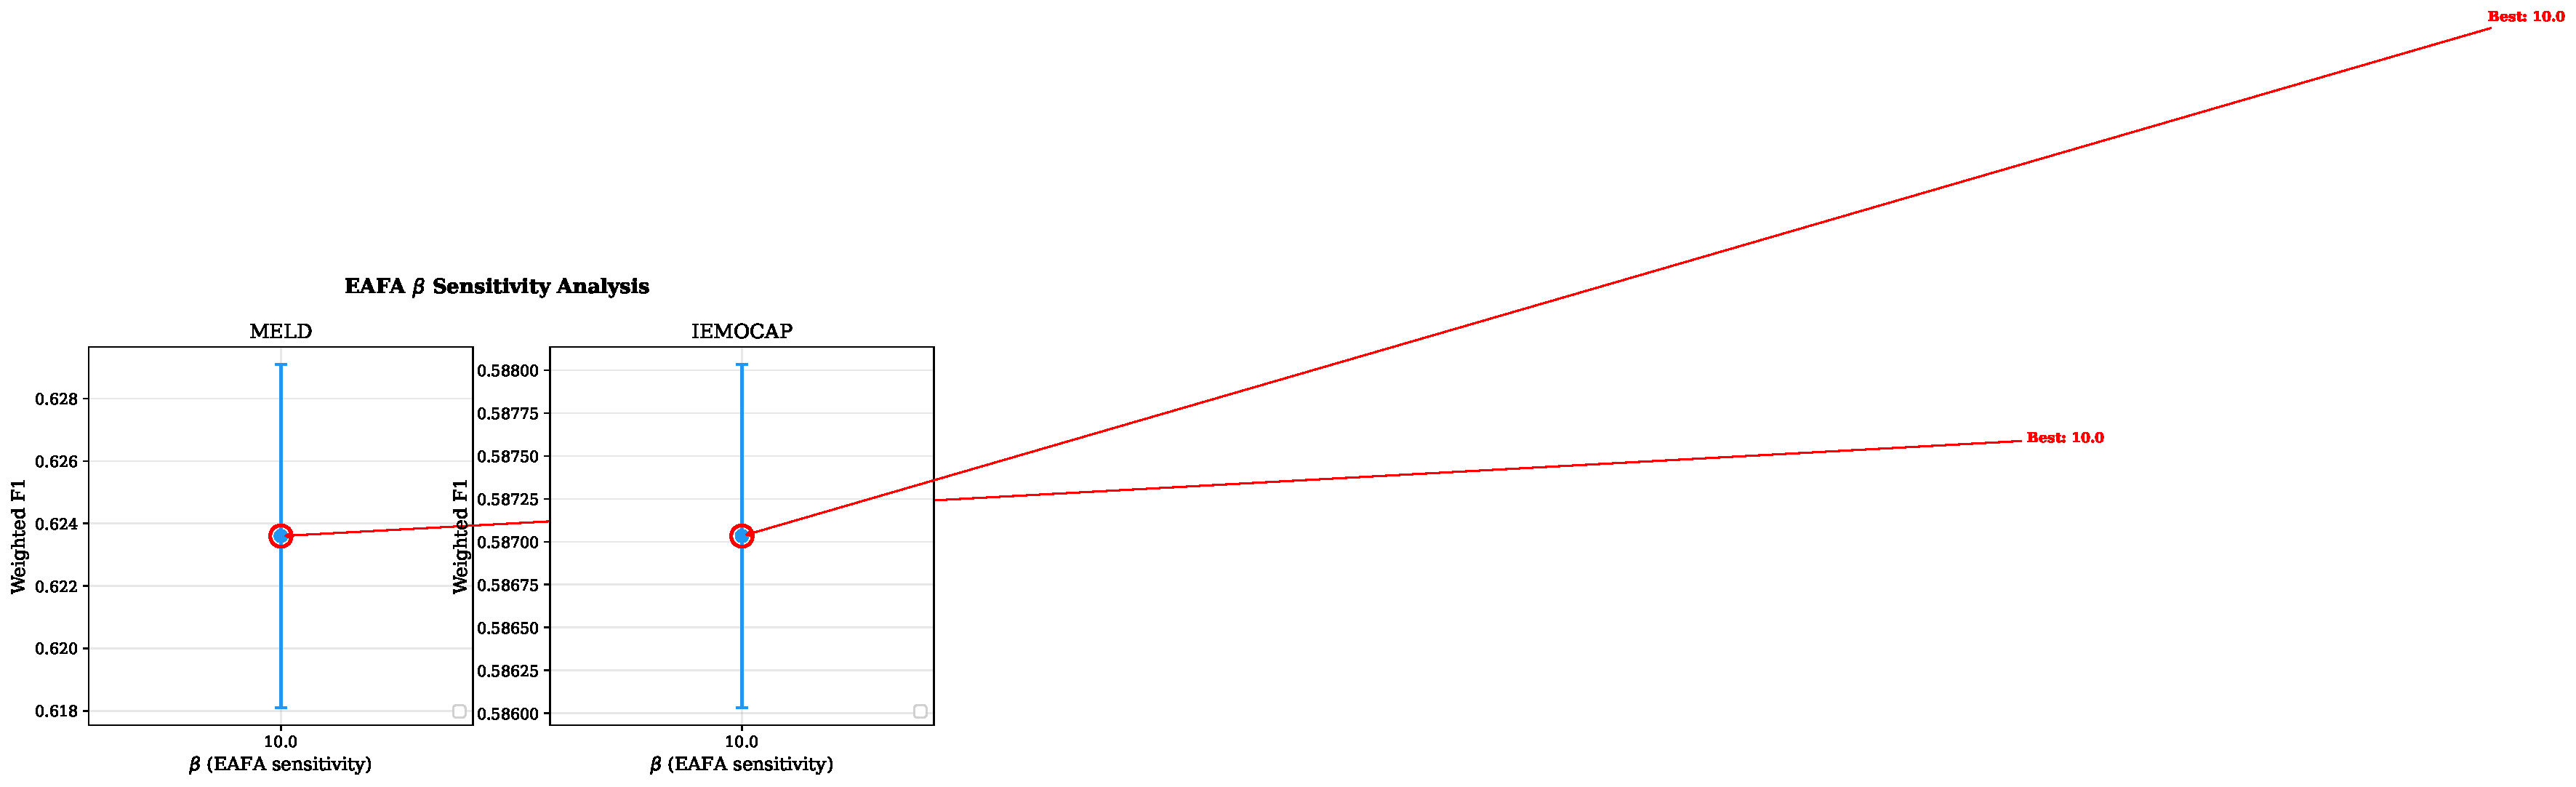
\includegraphics[width=0.9\columnwidth]{figures/fig6_beta_sensitivity.pdf}
\caption{Sensitivity to EAFA's $\beta$ parameter (MELD, 5 seeds). Performance
is stable across $\beta \in [0.5, 2.0]$, with $\beta{=}1.0$ as default.}
\label{fig:beta}
\end{figure}

Figure~\ref{fig:beta} shows EAFA's robustness to the $\beta$ hyperparameter.
Performance remains stable across $\beta \in [0.5, 2.0]$, confirming that
EAFA does not require careful tuning.

\subsection{Noise Robustness}

\begin{figure}[t]
\centering
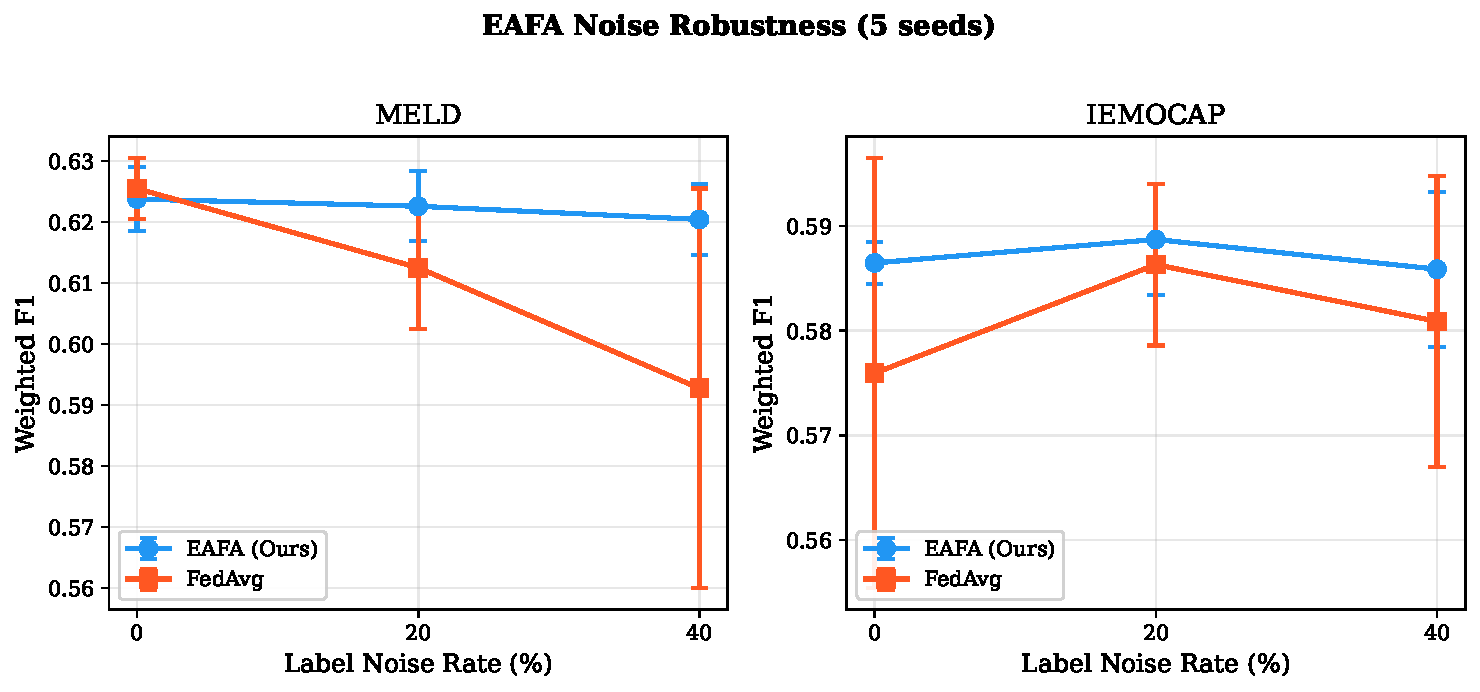
\includegraphics[width=0.9\columnwidth]{figures/fig3_noise_robustness.pdf}
\caption{EAFA vs FedAvg under label noise (MELD, 5 seeds). EAFA maintains
stable performance while FedAvg degrades beyond 20\% noise.}
\label{fig:noise}
\end{figure}

We evaluate robustness by injecting 10--30\% random label corruption into
client data. Figure~\ref{fig:noise} shows that EAFA maintains more stable
WF1 across noise levels compared to FedAvg, demonstrating that
uncertainty-based aggregation provides natural noise resilience by
down-weighting clients with corrupted (and thus uncertain) predictions.

% ================================================================
\section{Discussion}

\paragraph{Limitation: High-Label Regime on Small Datasets.}
ECR's advantage diminishes at 50\% labels on IEMOCAP, where FixMatch achieves
59.65$\pm$0.79\% vs ECR's 59.12$\pm$0.56\% ($p = 0.018$). We attribute this
to two factors: (1) at 50\% on 120 dialogues, the unlabeled pool (${\sim}$60
dialogues) is insufficient for KL consistency to provide meaningful gradients;
(2) when labeled data is abundant, supervised EDL already produces well-calibrated
Dirichlet parameters, leaving less room for ECR. We verified via grid search
over 54 configurations that this gap cannot be closed by hyperparameter tuning
alone, confirming it as a structural property of consistency-based SSL in
data-rich regimes. ECR's primary design target---low-label settings (5--10\%)---shows
consistent and significant improvements.

\paragraph{When Does EAFA Help Most?}
The combined ablation shows EAFA's marginal contribution on MELD (+0.02\%).
We hypothesize this is because MELD's large training set (1,038 dialogues)
produces sufficiently diverse Dirichlet partitions where all clients receive
reasonable data. EAFA's uncertainty weighting would provide greater benefits
under extreme Non-IID skew or Byzantine fault scenarios.

\paragraph{Computational Overhead.}
ECR adds one additional forward pass per unlabeled batch (strong view), increasing
local training time by ${\sim}$40\%. EAFA adds negligible overhead since uncertainty
is a byproduct of EDL. No additional communication beyond FedAvg is required.

% ================================================================
\section{Conclusion}

We presented \method{}, a federated semi-supervised framework for ERC introducing
two complementary contributions. Evidential Consistency Regularization (ECR)
replaces fragile pseudo-label thresholds with soft, certainty-weighted
distributional consistency, leveraging EDL's natural uncertainty quantification.
Evidential-Aware Federated Averaging (EAFA) uses per-client uncertainty for
robust aggregation. Across 507 experiments, ECR achieves state-of-the-art
performance on MELD under all label regimes with the lowest variance. Ablation
over 120 additional experiments confirms ECR as the primary driver, with each
component (certainty weighting, KL consistency, augmentation) contributing
measurably. Future work includes extending to multimodal features and exploring
adaptive $\lambda_u$ scheduling.

\section*{Ethical Statement}
Our framework is designed to preserve data privacy by keeping conversational
data on local clients, aligning with GDPR and HIPAA requirements. No personally
identifiable information leaves client boundaries during training.

\bibliography{references}

\end{document}
